
\section{Server-Client Synchronisation}

\newcommand{\stepOneName}{lockstep}
\newcommand{\stepTwoName}{simple server client}
\newcommand{\stepThreeName}{server client with simulation}

% topology of network(star diagram, what server does, what client does)
% protocol for synching game states between client server (command, update)
% advantages/disadvantages of lockstep
% advantages/disadvantages of server client with simulation


\begin{comment}

this section talks about the decision for server client architecture.
server-client allows master copy to exist on server.

- master copy of world on server
- clients perform no logic, only apply updates to

we need to work out how the computers talked to each other very early on
2 considerations: peer 2 peer, client-server
  - advantages of peer 2 peer
  - advantages of peer server-client
  - why server-client chosen 
  - issues experienced with server-client
    - jumpy ship movements
    

\end{comment}

The game was designed around being multiplayer, so our first goal was to decide how the player's computers would talk to each other.
Since their was an arbitrary number of players (greater than 1), We needed a system that would scale, but would also be robust.
The game was expecting all players to be on the same LAN (Local Area Network), hence a high bandwidth was available for the communications.

There are 3 strategies for the interactions between computers:
\begin{itemize}
\item \stepOneName
\item \stepTwoName
\item \stepThreeName
\end{itemize}

\begin{marginfigure}
	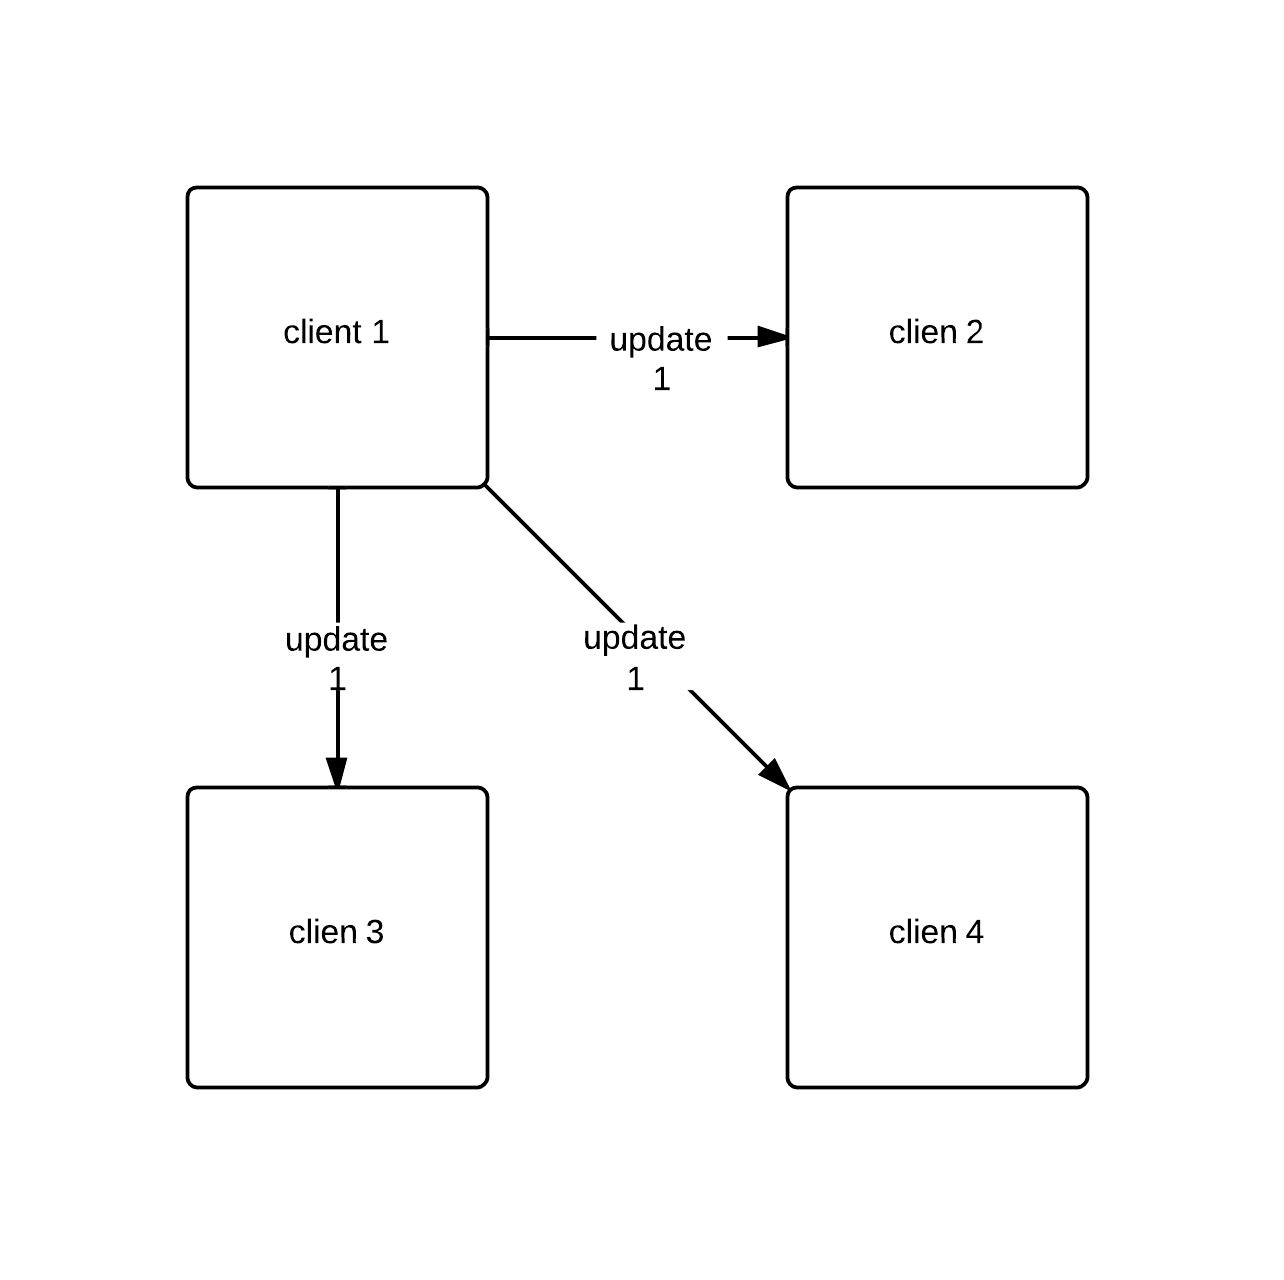
\includegraphics{res/computer_communication_architecture/ServerClientSynchronizationP2P.png}
	\caption{
	\stepOneName : 4 clients connected. client 1 has just modified its game state, so it send the update to all other clients.
	}
	\label{fig:serverClientSychP2P}
\end{marginfigure}

% what
\stepOneName is a peer to peer strategy, in which each computer has a full model of the game. Figure \ref{fig:serverClientSychP2P} shows an example of this strategy. 
Their are 4 computers within game. Each client (client 1, client 2, client 3, and client4) have a full copy of the game.
When client 1 updates performs some actions, they must update their game state, and send this update to all other clients.

\begin{marginfigure}[-30em]
	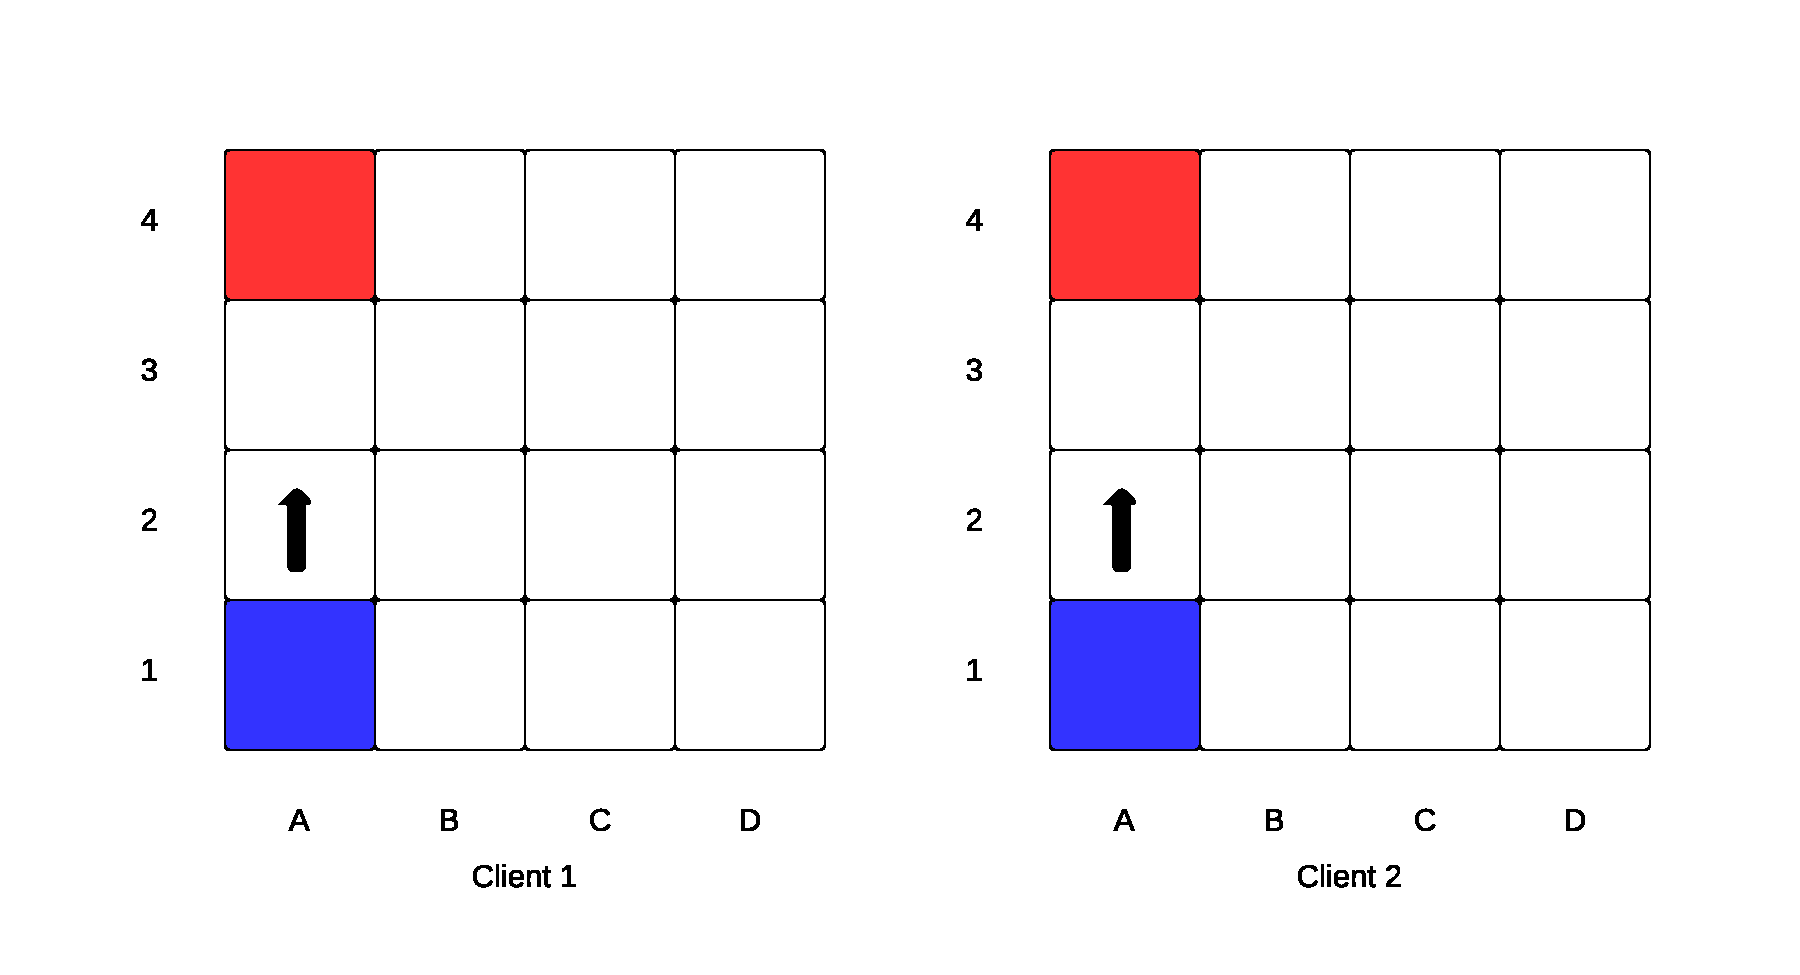
\includegraphics{res/computer_communication_architecture/ServerClientDesynchronisation1.pdf}
	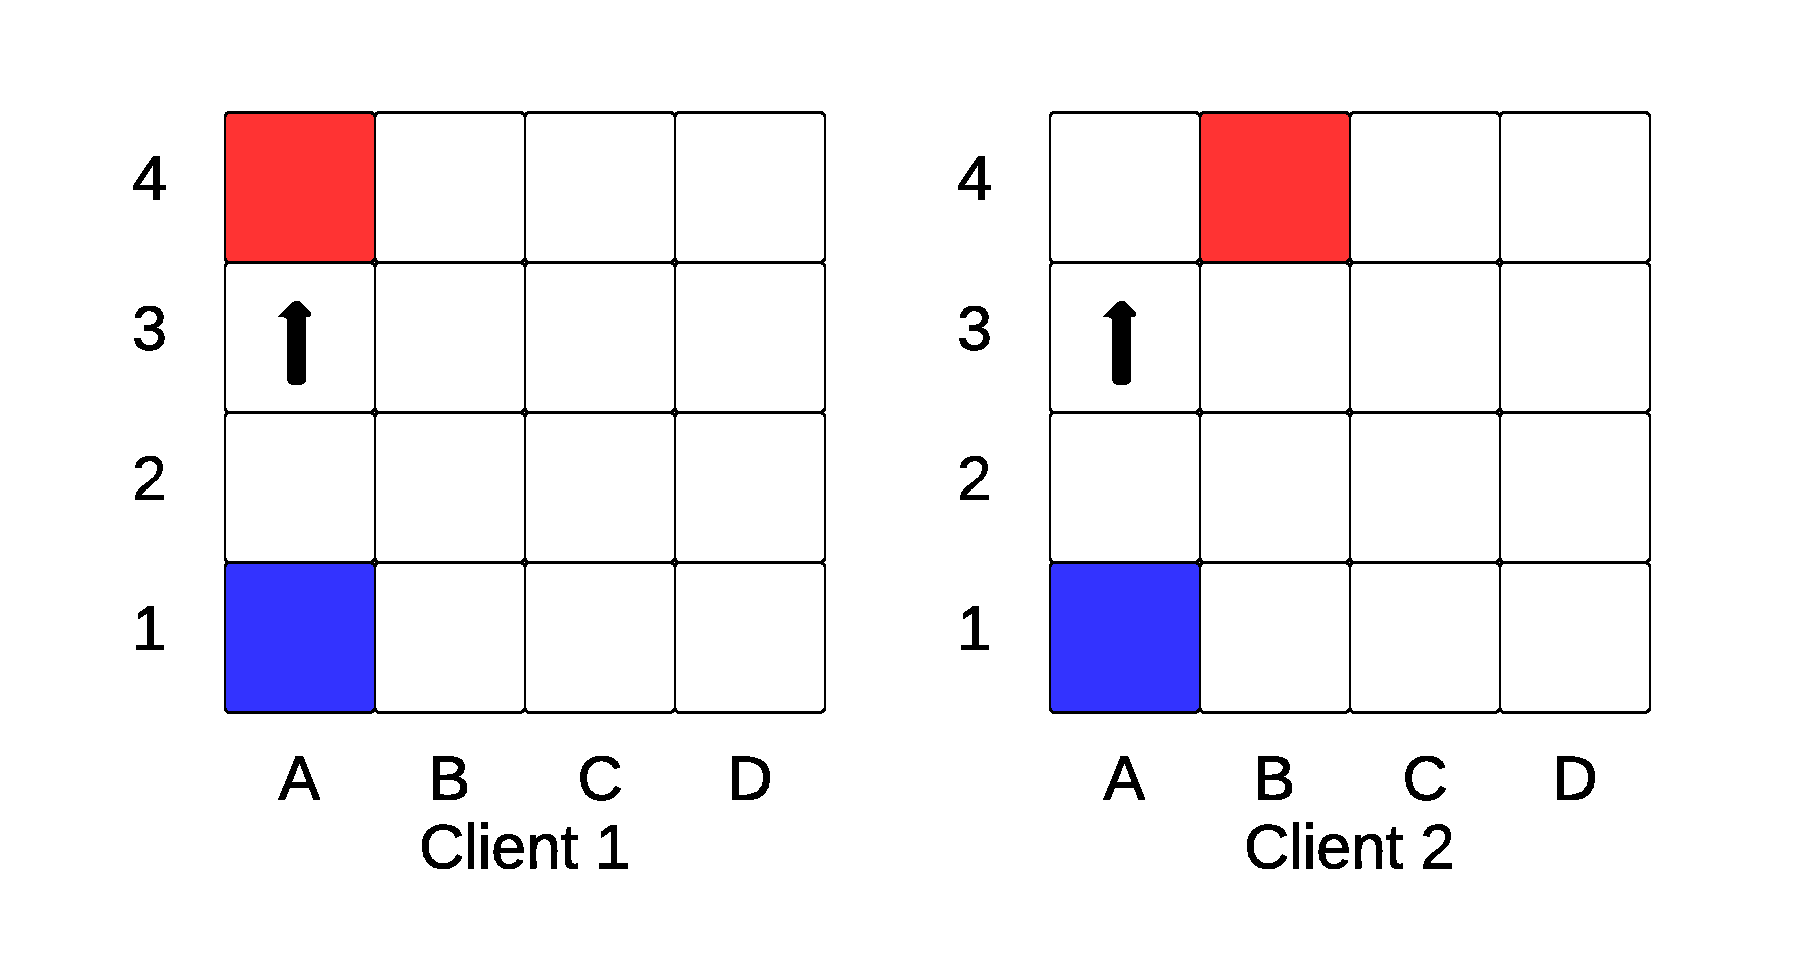
\includegraphics{res/computer_communication_architecture/ServerClientDesynchronisation2.pdf}
	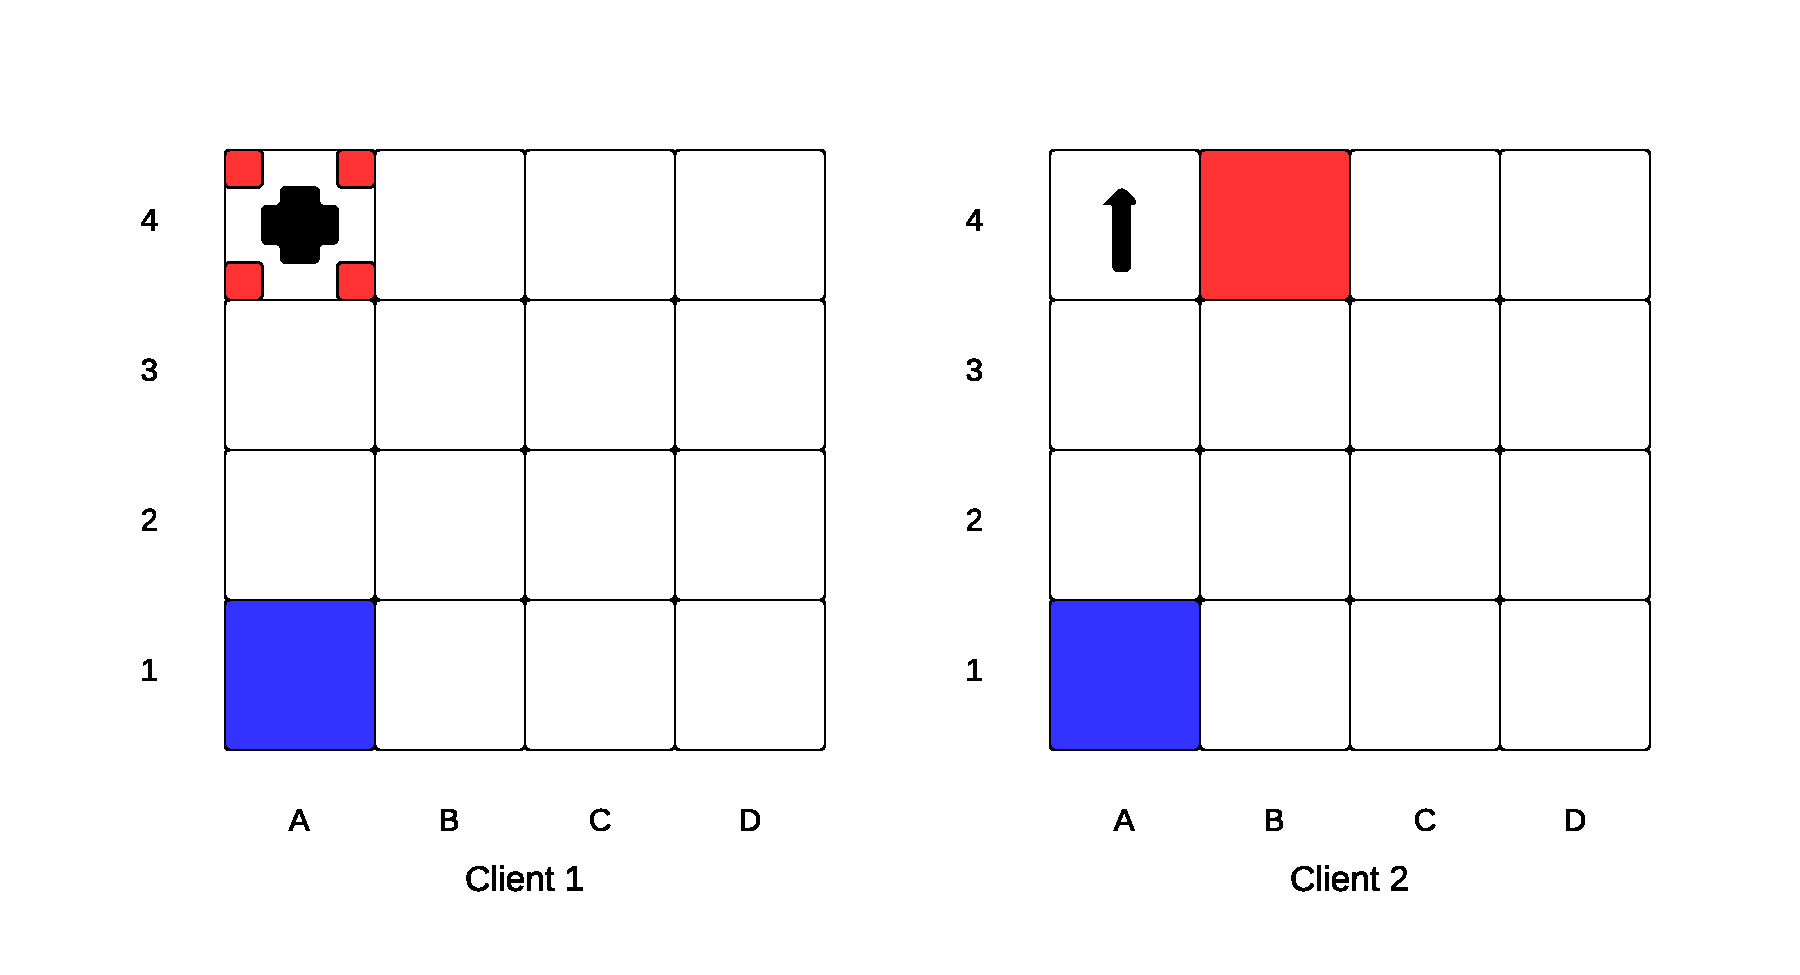
\includegraphics{res/computer_communication_architecture/ServerClientDesynchronisation3.pdf}		
	\caption{
	\stepOneName : example of desynchronization when using the \stepOneName strategy. Client 1 on left, client 2 on right. 
	Each diagram represents state of game for that clients at a given time period.	3 diagrams vertically aligned, First one is top, second one is middle, third one is bottom.
	}
	\label{fig:serverClientDesync}
\end{marginfigure}

% advantages
%   playable with slow networks
This strategy means players can continue to play games on networks with high latency, without any lag. When packets are delayed, the client can continue to play the game, and the game is updated when the packet arrives.
%   no dedicated server required
No client is picked to act as server, which causes game to end if that selected client disconnects.
Since all clients act as server, any client can disconnect and the game continues, providing more robustness which is highly desirable for games with long game intervals, such as Civilization series\cite{civilizationInMyPants}.



% disadvantages
%   disynchronization
Maintaining synchronisation when using a peer-2-peer protocol can be very challenging from a technical point of view, with non-determinism being caused by messages being received by clients at different times causing race conditions.
When this happens in a game, it can cause clients game states to desynchronise.
For example, In Figure \ref{fig:serverClientDesync}, there are 2 clients.
%   corrupted client can effect the entire game



% res/computer_communication_architecture




% lockstep
%   - each client has the master copy of the world
%   - when a client does something, it tells all others
%   - problems:
%     - desycnhronization
%     - currupted client fucks up everyone

% simple server client
%   - it's what we've implemented
%   - no simulation on clients
%   - 1 server that has master copy
%   - server does all processing and sends updates to clients
%   - clients just render the world and send commands to server

% server client with simulation
%   - similar to simple server client but client does 'some' simulation. They in no way can effect the world.
%   - for instance if client knows ships destination and current location it can render the ship graciously moving instead of jumping on every update.

